This is the dashboard subsystem where it will consist of a link to the Degree Planner, have the ability to view the flowchart of the chosen major, and will be able to sign in and sign out of the user account. 

\subsection{Homepage/Login}
Initially this page will look as the homepage, where the user will have the option to create an account or sign in. Once signed in, the page will turn into the dashboard, then they'll have the option of signing out.

\begin{figure}[h!]
	\centering
 	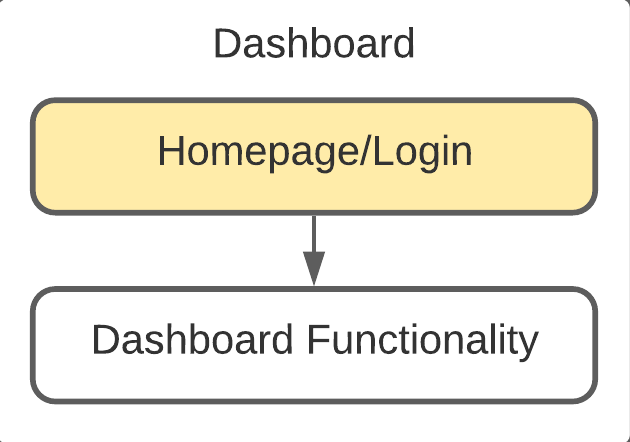
\includegraphics[width=0.60\textwidth]{images/Dashboard_Pic1}
 \caption{Homepage/Login}
\end{figure}

\subsubsection{Assumptions}
An assumption is the user isn't signed in so that means they can view the homepage, and the user is signed in to view the dashboard. 

\subsubsection{Responsibilities}
Initially when the user is not signed-in then there will be only the options of sign-in/create account where this will be shown as a homepage. Only when the user is signed in will the homepage be turned into the dashboard where the user can access other functions of it.

\subsubsection{Subsystem Interfaces}

\begin {table}[H]
\caption {Homepage/Login Subsystem interfaces} 
\begin{center}
    \begin{tabular}{ | p{1cm} | p{3cm} | p{5cm} | p{5cm} |}
    \hline
    ID & Description & Inputs & Outputs \\ \hline
    \#1 & Create an Account & \pbox{5cm}{Fill out given form\\Set Username and Password} & \pbox{3cm}{Account is Created}  \\ \hline
    \#2 & Sign in & \pbox{5cm}{Username and Password} & \pbox{5cm}{User will be Signed In}  \\ \hline
    \#3 & Sign Out & \pbox{5cm}{Click Sign Out button} & \pbox{5cm}{User will be Signed Out}  \\ \hline
    \end{tabular}
\end{center}
\end{table}

\subsection{Dashboard Functionality}
The dashboard will have a link to the Degree Planner functionality, then it will provide an option for the user to view their flowchart for the given major such as Software Engineering, and finally they will be able to sign out of their account.

\begin{figure}[h!]
	\centering
 	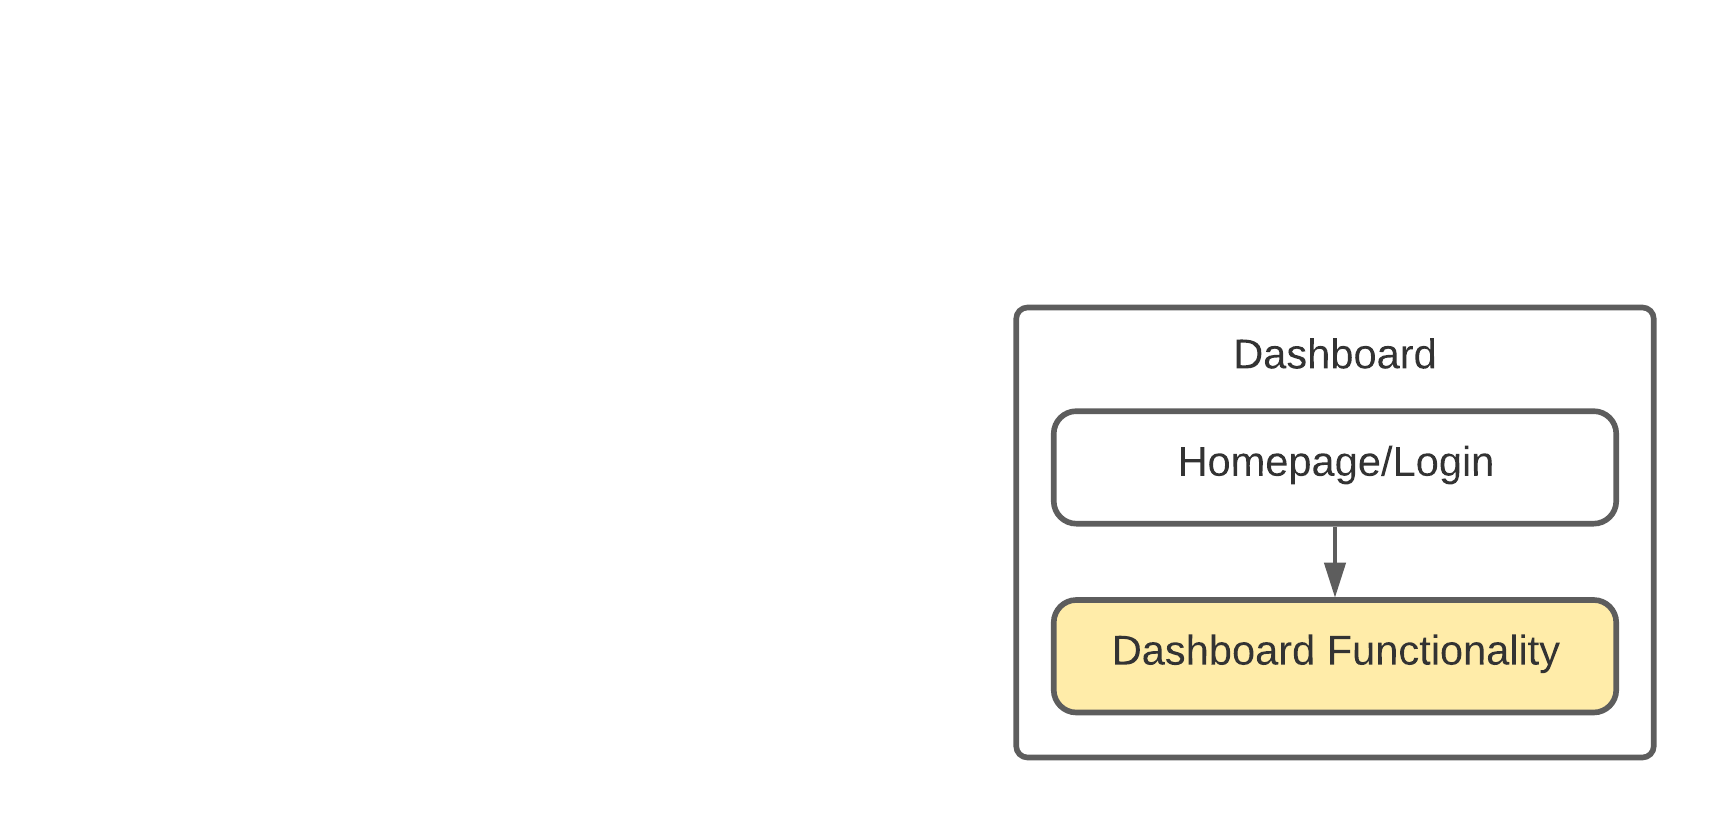
\includegraphics[width=0.60\textwidth]{images/Dashboard_Pic2}
 \caption{Dashboard Functionality}
\end{figure}


\subsubsection{Assumptions}
It is assumed that the user is already signed in so that they can access these features. 

\subsubsection{Responsibilities}
This will provide a link to access the degree planner GUI, then a option to view the flowchart of the chosen major, and also have the option of signing out. 

\subsubsection{Subsystem Interfaces}
\begin {table}[H]
\caption {Dashboard Functionality Subsystem interfaces} 
\begin{center}
    \begin{tabular}{ | p{1cm} | p{4cm} | p{4cm} | p{5cm} |}
    \hline
    ID & Description & Inputs & Outputs \\ \hline
    \#1 & Degree Planner Link & \pbox{3cm}{Click on Link} & \pbox{5cm}{Goes to Degree Planner}  \\ \hline
    \#2 & View Flowchart & \pbox{4cm}{Click on the Button} & \pbox{5cm}{Flowchart will be available}  \\ \hline
    \end{tabular}
\end{center}
\end{table}
